\textbf{GUI Implementation:}\\
The implementation was done in Visual Studios C\# 2010 using Windows Forms. The live view of the table and the option to select game and start recording can be seen in figure \ref{fig:guilive}. The history of the game and previous games can be seen in \ref{fig:guihist}. The figure \ref{fig:guisett} is the settings where the table can be calibrated by clicking a button and the balls by clicking on them. After calibration the settings can be saved and will be used as default when running the program in the futurs.

\begin{figure}[H]
\begin{center}
\leavevmode
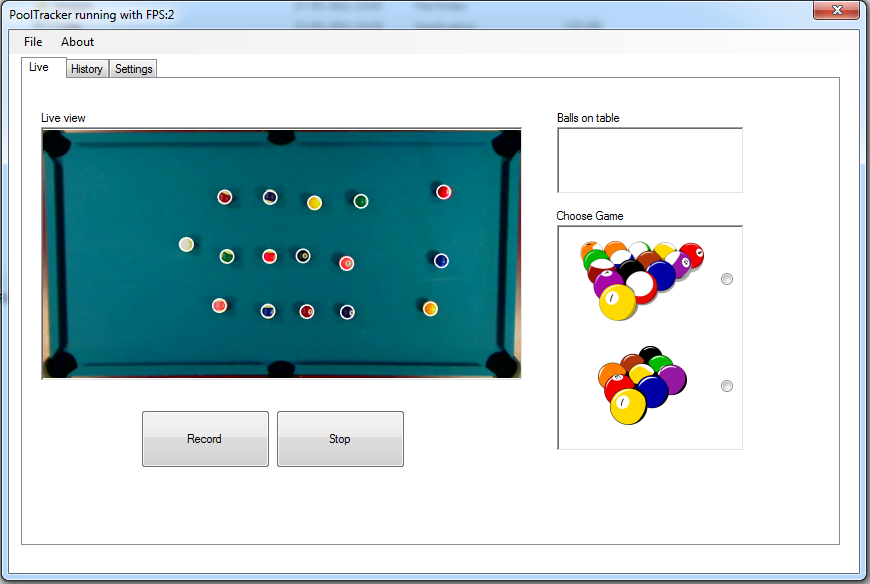
\includegraphics[width=0.7\textwidth]{images/prototype/live}
\end{center}
\caption{GUI: Live view tab.}
\label{fig:guilive}
\end{figure}

\begin{figure}[H]
\begin{center}
\leavevmode
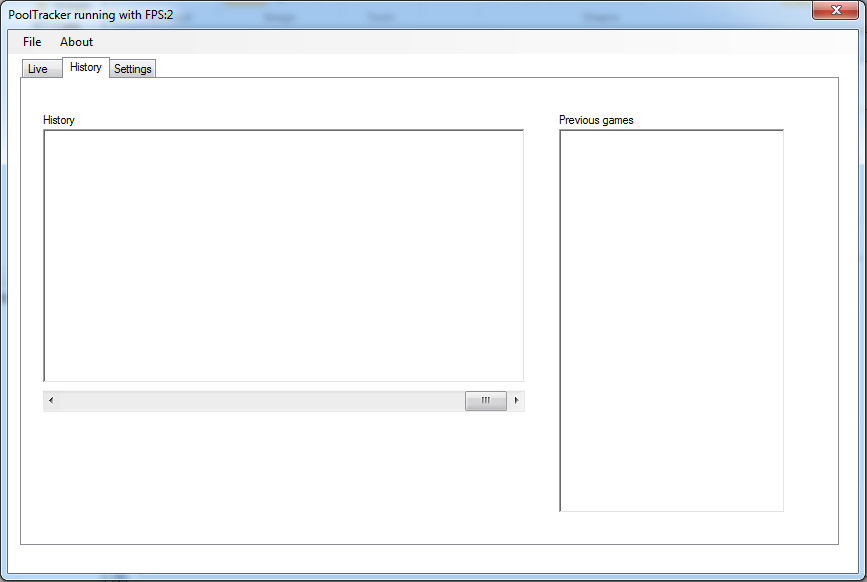
\includegraphics[width=0.7\textwidth]{images/prototype/hist}
\end{center}
\caption{GUI: History tab.}
\label{fig:guihist}
\end{figure}

\begin{figure}[H]
\begin{center}
\leavevmode
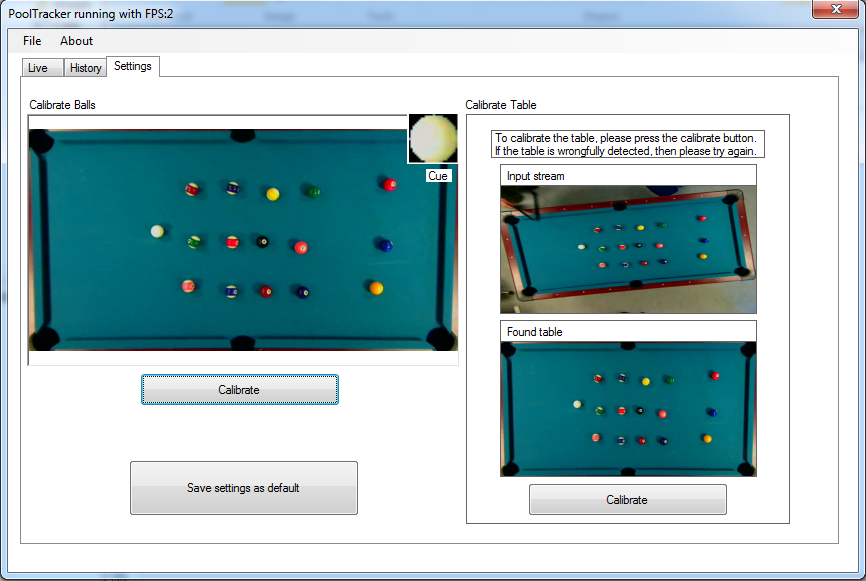
\includegraphics[width=0.7\textwidth]{images/prototype/settings}
\end{center}
\caption{GUI: Settings tab.}
\label{fig:guisett}
\end{figure}